\documentclass[12pt, oneside]{amsart}
\usepackage{amsmath}
\usepackage{lipsum}
\linespread{1.25}
\setlength{\topmargin}{0.in}
\setlength{\oddsidemargin}{0.33in}
\setlength{\textheight}{9.0in}
\setlength{\textwidth}{6.0in}
%-------Packages---------
\usepackage{amssymb,amsfonts}
\usepackage[all,arc]{xy}
\usepackage{enumerate}
\usepackage{mathrsfs}
\usepackage{graphicx}
\usepackage{epstopdf}
\usepackage{listings}
\usepackage{appendix}
\usepackage{listings}
\usepackage{placeins}
%\usepackage[square,numbers]{natbib}
\usepackage[style=apa,sortcites=true,sorting=nyt,backend=biber,natbib=true]{biblatex}
%bibliographystyle{unsrtnat}
\addbibresource{References/reference.bib}


%--------Theorem Environments--------
%theoremstyle{plain} --- default
\newtheorem{thm}{Theorem}[section]
\newtheorem{cor}[thm]{Corollary}
\newtheorem{prop}[thm]{Proposition}
\newtheorem{lem}[thm]{Lemma}
\newtheorem{conj}[thm]{Conjecture}
\newtheorem{quest}[thm]{Question}

\newtheorem{innercustomthm}{Theorem}
\newenvironment{customthm}[1]
  {\renewcommand\theinnercustomthm{#1}\innercustomthm}
  {\endinnercustomthm}

\theoremstyle{definition}
\newtheorem{defn}[thm]{Definition}
\newtheorem{defns}[thm]{Definitions}
\newtheorem{con}[thm]{Construction}
\newtheorem{exmp}[thm]{Example}
\newtheorem{exmps}[thm]{Examples}
\newtheorem{notn}[thm]{Notation}
\newtheorem{notns}[thm]{Notations}
\newtheorem{addm}[thm]{Addendum}
\newtheorem{exer}[thm]{Exercise}

\theoremstyle{remark}
\newtheorem{rem}[thm]{Remark}
\newtheorem{rems}[thm]{Remarks}
\newtheorem{warn}[thm]{Warning}
\newtheorem{sch}[thm]{Scholium}
\newcommand{\be}{\begin{equation}}
\newcommand{\ee}{\end{equation}}
\makeatletter
\let\c@equation\c@thm
\makeatother
\numberwithin{equation}{section}

%\bibliographystyle{plain}
%%%%%%%%%%%%%%%%%%%%%%%%%%%%%%%%%%%%%%%%%%%%%%%%%%%%%%%%%%%%%%%%%%%%%%%%%%%%%%%%%
% your title/author/date information go here
%--------Meta Data: Fill in your info------


\title{Cross-Validation Techniques for Auto-regressive Time Series}

\author{Xuan Li}

\date{September 24, 2024}

\begin{document}
\begin{abstract}
    This report is based on the paper "A Note on the Validity of Cross-Validation for Evaluating Autoregressive Time Series Prediction" \citep{Bergmeir2018}. There are three sections in this report. The first section provides a comprehensive summary of the paper \citep{Bergmeir2018}, presenting the key findings and some general perspectives toward understanding the work. The second section presents two possible research extension proposals beyond the original paper. The final section includes an extensional study we explore. In the study, we aim to mimic similar experiments using autoregressive models with an added lasso regression term, and we compare different cross-validation methods (including a blocked CV method) with out-of-sample estimation in terms of estimating the prediction error. Additionally, the proof of Theorem 1 in the original paper in this extensional scenario will be discussed from a general perspective.
\end{abstract}
\maketitle
\tableofcontents

%%%%%%%%%%%%%%%%%%%%%%%%%%%%%%%%%%%%%%%%%%%%%%%%%%%%%%%%%%%%%%%%%%%%%%%%%%%%%%%%%section 1

\section{Summary of the Original Paper}
The original paper demonstrates the validity of using $K-fold$ cross-validation (CV) methods for evaluating auto-regressive time series models \citep{Bergmeir2018}. Cross-validation is a widely used method in machine learning regression and classification problems \citep{Hastie}. However, for time series data, CV is often considered problematic due to the serial correlation and non-stationarity in the dependent data setting \citep{Bergmeir2012}. The authors demonstrated that cross-validation methods can be valid and effective for auto-regressive models under certain conditions \citep{Bergmeir2018}. The results are shown through both the theoretical proof and practical simulations. \\

The paper builds on the existing literatures on for time series data model fitting techniques. Traditionally, out-of-sample ($OOS$) evaluation is preferred for time series due to concerns about using the future data to predict the past data, and issues with correlation in errors \citep{Bergmeir2018}. In $OOS$, a block of data at the end of the set is left out as the testing data, and the remaining data is used as the training data. There are many studies that demonstrate this procedure \citep{Tashman}. Previous studies have also proposed different modifications to CV to adapt for the dependent data setting \citep{Gyorfi, Burman1992, Burman1994}, such as $h-block$ CV \citep{Burman1994}. In $h-block$ CV, $h$ data points preceding and following the testing data are left out in the training set due to avoiding dependency. The authors of the original paper \citep{Bergmeir2018} referred to this type of CV as non-dependent cross-validation $nonDepCV$. However, this procedure often leads to inefficient use of data. The authors present their work as a shift from the conventional thinking by demonstrating that the standard $K-fold$ CV is not only valid but also helpful for auto-regressive models under certain conditions. In this case, the $K-fold$ CV can be used without modification, i.e., future data can be used as training data and past data can be used as testing data during this procedure. This is a key contribution of the paper. It challenges the conventional thinking that CV is not appropriate for time series data. \\

The main idea is that the error result we get by performing cross validation methods on a data set $\{y_t\}_{t=1}^T$, denoted as $\hat{PE}$, can approximate the prediction error when forecasting on a future data set $\{y_t\}_{T+1}^n$, denoted as $PE$. 

\subsection{Theoretical Work}
The original paper provides a theoretical proof by showing that the prediction error on the in-set data performed by CV is a consistent estimator for the prediction error on the out-set data (the unseen future data). Without loss of generality, the paper's theoretical proof focuses on the leave-one-out CV ($LOOCV$) scene since generalisation to the $K-fold$ CV is straightforward.
\\

Let $y_1, y_2, ..., y_n$ be a set of observation data from a stationary process. Let's consider a purely auto-regressive model of order $P$, i.e., AR(p), consider the following nonlinear regression model
\begin{equation}\label{eq1}
y_t = g(x_t, \theta) + \epsilon_t
\end{equation}

where $\epsilon_t$ is the regression error term, $x_t$ consists the lagged values of $y_t$ and $\theta$ is the parameter vector with all the coefficients values, and $g$ is the function of the lagged values of $y_t$ up to $p^{th}$ order.  $g$ is a continuous and differentiable function with respect to $\theta$ for all $x_t$ = $(y_{t-1}, y_{t-2}, ..., y_{t-p})'$. The estimation of $\hat{\theta}$ is the argument that minimises the objective function
\begin{equation}\label{eq2}
Q(\theta) = \sum_{t=p+1}^{n}
(y_t - g(x_t, \theta))^2
\end{equation}

Now suppose that $\{\Tilde{y_t}\}^m_{t=1}$ is another set of observations that has the same distribution as $\{{y_t}\}^n_{t=1}$, which can be the future data
\begin{equation}\label{eq3}
\Tilde{y_t} = g(\Tilde{x_t}, \theta) + \Tilde{\epsilon_t}
\end{equation}
The prediction error is defined as
\begin{equation}\label{eq4}
    PE = E(\Tilde{y} - g(\Tilde{x},\hat{\theta})^2
\end{equation}
where $\hat{\theta}$ here is the estimate minimizing the objective function $\tilde{Q}(\theta) = \sum_{t=p+1}^{m}
(\tilde{y}_t - g(\tilde{x}_t, \theta))^2$.
In the paper, the authors consider estimating $PE$ on dataset $\{\Tilde{y_t}\}^m_{t=1}$ by performing cross-validation on $\{y_t\}^n_{t=1}$. In the $LOOCV$ scene,  the training sample is $\{(x_j
, y_j); j = p+1,...,n, j \not = t\}$ and the test sample is $\{(x_t
, y_t)$\}. The estimator of $PE$ (denoted by $\hat{PE}$)  is defined as
\begin{equation}\label{eq5}
\hat{PE} = \frac{1}{n-p} \sum_{t=p+1}^n \left( y_t - g(x_t,\hat{\theta_{-t}}) \right)^2
\end{equation}
where $\hat{\theta_{-t}}$ is the leave-one-out estimate for $\theta$ on $\{(x_j, y_j); j = p+1,...,n, j \not = t\}$. In order to prove that $\hat{PE}$ approximates $PE$, the following assumptions are needed.

\newtheorem{assumption}{Assumption}
\begin{assumption}\label{assump1}
    The nonlinear AR(p) process that generated $\{{y_t}\}^n_{t=1}$ is stationary and ergotic.
\end{assumption}

\begin{assumption}\label{assump2}
    $\hat{\theta_{-t}}$ is a consistent estimator of $\theta$.
\end{assumption}


\begin{assumption}\label{assump3}
The errors are MDS: 
\begin{enumerate}
    \item $ \{ \epsilon_t,F_t \}$ form a sequence of martingale differences (MDS) where $F_t$ is the sigma field generated by $ \{ \epsilon_s, y_s;s \leq t \} $. Note that i.i.d errors are MDS.
    \item $Var(\epsilon_t | x_t) = \sigma^2$ and $E[|\epsilon_t|^{4+\delta} < K$ for some $K < \infty$ and $\delta > 0$.
    \item $\{\epsilon_t\}$ have absolutely continuous distribution with respect to Lebesgue measure. 
\end{enumerate}
\end{assumption}

Note that due to stationarity of $\{y_t\}^n_{t=1}$, conditions for the consistency of $\hat{\theta}$ and $\hat{\theta_{-t}}$ are equivalent. In short, we want to make sure that the time series model is stationary, the estimator is consistent, and the errors are uncorrelated.  \\

The theoretical validity is carried out by proving the following theorem. Compared to the original paper, we have slightly altered the notation for better clarification in the proof, and we also restructured the proof by introducing some additional notation, which makes the logic easier to follow.

\begin{customthm}{1}\label{thm1}
Suppose that Assumptions \ref{assump1}-\ref{assump3} hold, then we have $\hat{PE} \xrightarrow[]{approx.} PE$. 
\end{customthm}
\begin{proof}
    
By expanding the prediction error into integral form, we have
$$PE = \int (\Tilde{y} - g(\Tilde{x},\hat{\theta}))^2 d\Tilde{F_m}$$
where $\Tilde{F_m}$ is the distribution of the process generating $\{\Tilde{y_t}\}^m_{t=1}$. Suppose the true model is $\Tilde{y} = g(\Tilde{x}, \theta) + \Tilde{\epsilon}$, where $g(\Tilde{x}, \theta)$ represents the true underlying relationship between $\Tilde{x}$ and $\Tilde{y}$, and $\Tilde{\epsilon}$ is the noise. By substituting for $\Tilde{y}$, we have 
$$PE = \int \left( g(\Tilde{x}, \theta) + \Tilde{\epsilon} - g(\Tilde{x},\hat{\theta}) \right)^2 d\Tilde{F_m}$$ By expanding the squared terms and simplification, we have 
$$PE = \int \left[ (g(\Tilde{x}, \theta) - g(\Tilde{x},\hat{\theta}))^2 + \Tilde{\epsilon}^ 2 \right] d\Tilde{F_m}$$

The authors performed a bias-variance decomposition by subtracting and adding the expected prediction $E[g(\Tilde{x}, \hat{\theta})]$, which represents the average prediction over multiple realizations of the training data. Therefore, we have 
$$ PE = \int \left[ \left(g(\Tilde{x}, \theta) - E[g(\Tilde{x}, \hat{\theta})] + E[g(\Tilde{x}, \hat{\theta})] - g(\Tilde{x},\hat{\theta})\right)^2 + \Tilde{\epsilon}^2 \right] d\Tilde{F_m}$$ By expanding the squared terms, we have

\begin{align*}
    PE &= \int \bigg[ \left(g(\tilde{x},\theta) - E[g(\tilde{x},\hat{\theta})]\right)^2 + \left(E[g(\tilde{x},\hat{\theta})] - g(\tilde{x}, \hat{\theta})\right)^2 \\
    &+ 2 \left( g(\tilde{x}, \theta) - E[g(\tilde{x}, \hat{\theta})]\right) \left( g(\tilde{x},\hat{\theta}) - E[g(\tilde{x}, \hat{\theta})] \right) + \tilde{\epsilon}^2 \bigg] d\Tilde{F_m} 
\end{align*}

Notice that the cross-term vanishes when integrated since $E[ g(\tilde{x},\hat{\theta}) - E[g(\tilde{x},\hat{\theta}))] = 0$, and hence the equation can be simplified to
\begin{align*}
PE  &= \int \left[ \left(g(\Tilde{x}, \theta) - E[g(\Tilde{x}, \hat{\theta})] \right)^2 + \left(E[g(\Tilde{x}, \hat{\theta})] - g(\Tilde{x},\theta)\right)^2 + \Tilde{\epsilon}^2 \right] d\Tilde{F_m}\\ 
    &= \underbrace{\int  \left(g(\Tilde{x}, \theta) - E[g(\Tilde{x}, \hat{\theta})] \right)^2 d\Tilde{F_m}}_\text{Bias} + \underbrace{\int \left(E[g(\Tilde{x}, \hat{\theta})] - g(\Tilde{x},\hat{\theta})\right)^2 d\Tilde{F_m}}_\text{Variance} + \underbrace{\int \Tilde{\epsilon}^2  d\Tilde{F_m}}_\text{noise}\\  
\end{align*}
We expand $\hat{PE}$ in a similar vein. 
\begin{align*}
     \hat{PE} = \underbrace{\int  \left(g(x, \theta) - E[g(x, \hat{\theta_{-t}})] \right)^2 dF_n}_\text{Bias} + \underbrace{ \frac{1}{n-p}\sum_{t=p+1}^n \left( E[g(x_t, \hat{\theta_{-t}})] - g(x_t, \hat{\theta_{-t}}) \right)^2     }_\text{Variance} + \underbrace{\int \epsilon^2dF_n}_\text{noise}\\  
\end{align*}

where $F_n$ is the distribution of the process generating $\{y_t\}^n_{t=1}$. Notice that $\tilde{F_m}$ and $F_n$ are the empirical distributions of $2$ different samples from the same underlying process $F$, i.e $\{\Tilde{y_t}\}_{t=1}^m$ and $\{y_t\}_{t=1}^n$ are 2 datasets from the same underlying distribution process. By \textbf{Assumption \ref{assump1}} and \textbf{Assumption \ref{assump2}}, the underlying distribution process is stationary and ergotic, and  both $\hat{\theta}$ and $\hat{\theta_{-t}}$ are consistent estimators. The bias and noise terms in both $\hat{PE}$ and $PE$ are asymptotically identical. As $n, m \rightarrow \infty $, we want to show that

\begin{equation}\label{equation6}
   \frac{1}{n-p}\sum_{t=p+1}^n \left( E[g(x_t, \hat{\theta_{-t}})] - g(x_t, \hat{\theta_{-t}}) \right)^2 \xrightarrow{Approxi.} \int \left(E[g(\Tilde{x}, \hat{\theta})] - g(\Tilde{x},\hat{\theta})\right)^2 d\tilde{F_m} 
\end{equation}

The key takeaway here is that, ultimately, the variance of the true prediction error denoted by $PE$ is consistently estimated by the variance of the cross-validation prediction error $\hat{PE}$, when the number of data gets big. When $n, m$ becomes big, let $N = max \{n, m\}$, and let $\epsilon^E_t(\hat{\theta_{-t}}) = E[g(x_t, \hat{\theta_{-t}})] - g(x_t,\hat{\theta_{-t}}), \tilde{\epsilon}^E_t(
\hat{\theta}
) = E[g(\Tilde{x_t}, \hat{\theta})] - g(\Tilde{x_t},\hat{\theta})$, we can write the left term in equation \ref{equation6} as
$$  \frac{1}{N-p} \sum_{t=p+1}^N  \left( \epsilon^E_t(\theta_{-t}) \right)^2$$and similarly we can write the right term as $$  \frac{1}{(N-p)^2} \sum_{t=p+1}^N \sum_{j=p+1}^N  \tilde{\epsilon}^E_t(\hat{\theta}) \tilde{\epsilon}^E_j(\hat{\theta})$$
Our proof is complete if we can show that, as $N$ grows big
$$E\left[ \sum_{t=p+1}^N \sum_{j=p+1}^N  \tilde{\epsilon}^E_t(\hat{\theta}) \tilde{\epsilon}^E_j(\hat{\theta}) \right]  \approx E\left[\sum_{t=p+1}^N  \left( \epsilon^E_t(\theta_{-t}) \right)^2 \right]  $$ 
which follows by Lemma \ref{lemma1}. 
\end{proof}

\newtheorem{lemma}{Lemma}
\begin{lemma}\label{lemma1}
    Suppose that \textbf{Assumptions \ref{assump1}-\ref{assump3}} hold. Then, there exists an arbitrarily small constant c \textgreater 0 such that $$E \left[  \sum_{t=p+1}^N \sum_{j=p+1}^N   \tilde{\epsilon}^E_t(\hat{\theta}) \tilde{\epsilon}^E_j(\hat{\theta}) - \sum_{t=p+1}^N  \left( \epsilon^E_t(\theta_{-t}) \right)^2 \right]^4 \leq cN^4$$
\end{lemma}

\begin{proof}
Note that 

\begin{align*}
    &\sum_{t=p+1}^N \sum_{j=p+1}^N   \tilde{\epsilon}^E_t(\hat{\theta}) \tilde{\epsilon}^E_j(\hat{\theta}) - \sum_{t=p+1}^N  \left( \epsilon^E_t(\theta_{-t}) \right)^2 \\
    &= \underbrace{\sum_{t=p+1}^N (\tilde{\epsilon}^E_t(\hat{\theta}))^2 - \sum_{t=p+1}^N ( \epsilon^E_t(\hat{\theta_{-t}})) ^2}_\text{part 1} + \underbrace{\sum^N_{t=p+1, t\not = j} \sum^N_{j=p+1} \tilde{\epsilon}^E_t(\hat{\theta}) \tilde{\epsilon}^E_j(\hat{\theta})}_\text{part 2}
\end{align*} 

By adding and subtracting the expectation terms, we can express (part 1) of the above equation as
\begin{align*}
    \sum_{t=p+1}^N (\tilde{\epsilon}^E_t(\hat{\theta}))^2 - \sum_{t=p+1}^N ( \epsilon^E_t(\hat{\theta_{-t}})) ^2 
    & = \sum_{t=p+1}^N \left( (\tilde{\epsilon}^E_t(\hat{\theta}))^2 - E[(\tilde{\epsilon}^E_t(\hat{\theta}))^2] \right) \\
    &- \sum_{t=p+1}^N \left( ( \epsilon^E_t(\hat{\theta_{-t}}))^2 - E[( \epsilon^E_t(\hat{\theta_{-t}}))^2] \right) \\
    &+ \sum^N_{t=p+1} \left( E[(\tilde{\epsilon}^E_t(\hat{\theta}))^2] - E[( \epsilon^E_t(\hat{\theta_{-t}}))^2] \right) \\
    & \leq cN^2
\end{align*}
This is because that the summations here are martingale difference sequences (\textbf{Assumption \ref{assump3}}). Therefore by Burkholder's inequality, we have 
$$ E \Bigg|
\sum_{t=p+1}^N \left( (\tilde{\epsilon}^E_t(\hat{\theta}))^2 - E[(\tilde{\epsilon}^E_t(\hat{\theta}))^2] \right) \Bigg| ^4 \leq 
 c * E \Bigg|
\sum_{t=p+1}^N \left( (\tilde{\epsilon}^E_t(\hat{\theta}))^2 - E[(\tilde{\epsilon}^E_t(\hat{\theta}))^2] \right)^2 \Bigg| ^2 \leq cN^2 $$

$$ E \Bigg|
\sum_{t=p+1}^N \left( ( \epsilon^E_t(\hat{\theta_{-t}}))^2 - E[( \epsilon^E_t(\hat{\theta_{-t}}))^2] \right) \Bigg| ^4 \leq 
 c * E \Bigg|
\sum_{t=p+1}^N \left( ( \epsilon^E_t(\hat{\theta_{-t}}))^2 - E[( \epsilon^E_t(\hat{\theta_{-t}}))^2] \right)^2 \Bigg| ^2 \leq cN^2
$$

$$ E \Bigg|
\sum_{t=p+1}^N \left( E[(\tilde{\epsilon}^E_t(\hat{\theta}))^2] - E[( \epsilon^E_t(\hat{\theta_{-t}}))^2] \right) \Bigg| ^4 \leq 
 c * E \Bigg|
\sum_{t=p+1}^N \left( E[(\tilde{\epsilon}^E_t(\hat{\theta}))^2] - E[( \epsilon^E_t(\hat{\theta_{-t}}))^2] \right)^2 \Bigg| ^2 \leq cN^2
$$

For the (part 2) of the equation, due to the symmetry of a covariance matrix, we can express it as
$$\sum^N_{t=p+1, t\not = j} \sum^N_{j=p+1} \tilde{\epsilon}^E_t(\hat{\theta}) \tilde{\epsilon}^E_j(\hat{\theta}) = 2 
\sum^N_{t=p+2}\tilde{\epsilon}^E_t(\hat{\theta}) 
\sum^{j < t}_{j=p+1} \tilde{\epsilon}^E_j(\hat{\theta}) \leq cN^4
$$
This is because that sum of the off-diagonal elements of the variance-covariance matrix becomes negligible (the impact of the covariance terms becomes negligible). Note that both $\{ \tilde{\epsilon}^E_t  \}$ and $\{\epsilon^E_t\}$ are stationary martingale difference sequences, and any linear combination of martingales based on the same filtration is also a martingale. After omitting certain rows and applying the law of iterated expectation, this inequality follows from the proof of Lemma 5.3 in \citep{Burman1992}. And therefore, we have Lemma \ref{lemma1} proved. \end{proof}
\\

Note that \textbf{Errors are uncorrelated} will be the key component for the success of the cross-validation. In fact, as stated by the authors, the proposed CV method works exactly towards ensuring the uncorrelatedness between residuals. Alternatively, we can understand the proof from the perspective of the Glivenko-Cante's theorem in dependent setting. The theorem states that the empirical distribution function converges uniformly to the true distribution function under certain conditions \citep{Doukhan, Bradley}. In our case, the set of observations $\{y_t\}_{t=1}^n$ is generated from a stationary and ergotic process by \textbf{Assumption \ref{assump1}}. Due to stationarity, the dependence between observations decays exponentially (i.e the auto-correlations decay exponentially \citep{Takemura2016} for stationary AR processes),  and therefore indicates a $\alpha$-mixing condition \citep{Brockwell}. This was also mentioned by the authors in the original paper. Therefore, the data process in this case satisfies all conditions needed to apply the dependent version of Glivenko-Cante's theorem. Similar logic follows for $\{\tilde{y_t}\}_{t=1}^m$. Therefore, both $F_n$ and $\tilde{F_m}$ are empirical distribution functions of the observations $\{y_t\}_{t=1}^n$ and $\{\tilde{y_t}\}_{t=1}^m$ from the same underlying AR(p) process that satisfies the stationarity and mixing condition. By Glivenko-Cante's theorem, they converges uniformly to the true distribution function $F$ as the sample size grows large. 

\subsection{Generalization of Theorem 1}
Notice that in the proof, we did not rely on any specific properties of the AR(p) model itself. In \textbf{Assumption \ref{assump1}}, what truly matters are the stationarity and the alpha-mixing condition. Both of them can be extended to a wide range of time series models. \textbf{Assumption \ref{assump2}} ensures that we have consistent estimators for the coefficients terms. And \textbf{Assumption \ref{assump3}} (error terms form a martingale difference sequence) plays an important role in the proof as mentioned before. Both \textbf{Assumption \ref{assump2} and \ref{assump3}} do not depend on any specific properties of the AR(p) model, and they can be extended to a wide range of time series models as well. \\

Therefore, since the proof for \textbf{Theorem \ref{thm1}} depends on these general conditions (not on any special properties of the AR(p) model), we can extend the \textbf{Theorem \ref{thm1}} to a more general setting. By generalizing \textbf{Assumption 1}, we can apply the results of the cross-validation (CV) procedure beyond just the auto-regressive (AR) models. This can include any nonlinear time series models that meet the adjusted \textbf{Assumption 1} (i.e., \textbf{Assumption \ref{assump4}}), \textbf{Assumption 2}, and \textbf{Assumption 3}. 

\begin{assumption}\label{assump4}
    The generalized version of \textbf{Assumption 1} for any nonlinear time series process:
\begin{enumerate}
    \item \textbf{Stationarity}: The time series process should be stationary, so the statistical properties remain consistent over time.
    \item \textbf{Alpha-Mixing}: The process should satisfy the alpha-mixing condition, ensuring weak dependence between observations.
    \item \textbf{Correct Model Specification}: The model used for cross-validation must be correctly specified, meaning that it matches with the true data-generating process and therefore doesn't introduce bias due to misspecification.
\end{enumerate}
\end{assumption}
The martingale difference property of the error term in Assumption \ref{assump3} ensures that the errors are uncorrelated. It is key for the consistency and accuracy of the cross-validation error estimates. If the model is misspecified, it would cause correlations in the errors, which is why we account for this in the updated version of \textbf{Assumption \ref{assump1}}, i.e., \textbf{Assumption \ref{assump4}}. \\

In short, with Assumptions \textbf{\ref{assump2}-\ref{assump4}}, we can now apply \textbf{Theorem \ref{thm1}} to not only AR(p) models, but any nonlinear time series models.


\subsection{Monte Carlo Simulation and Results}
The authors demonstrate through R that $K-fold$ CV and $LOOCV$ outperform other approaches, using both general AR(p) and non-parametric models. The simulation contains 1000 Monte Carlo trials for three experiments: data-generating processes from AR(3), invertible MA(1), and seasonal AR(12) (this is a counter-example where CV fails). In each Monte Carlo trial, the time series data has length 200, with 70\% being used as in-set (for $\hat{PE}$) and 30\% hidden as out-set (for $PE$).\\

The methods used and compared are $5-fold$ CV, $LOOCV$, $nonDepCV$, and $OOS$ evaluation. For model fitting, the authors use linear AR models with up to 5 lags and a neural network (MLP) model with 5 hidden units.
To see how $\hat{PE}$ approximates $PE$, the authors use \textbf{mean absolute prediction accuracy error} and \textbf{mean prediction accuracy error}, i.e., $MAPAE = \frac{1}{k} \sum_j^k | \hat{PE}_j - PE_j|, MPAE = \frac{1}{k} \sum_j^k ( \hat{PE}_j - PE_j)$.
\textbf{Root mean squared error} and \textbf{mean absolute error} are used to evaluate for the out-set error, i.e., $RMSE = \frac{1}{N-T} \sum_{t=T}^N \sqrt{(y_t - g(x_t, \hat{\theta})^2}, MAE = \frac{1}{N-T} \sum_{t=T}^N |y_t - g(x_t, \hat{\theta}|$. Similarly, for consistency, the in-set error measures also use \textbf{RMSE} and \textbf{MAE}.\\

The results show that $5-fold$ CV and $LOOCV$ outperform $OOS$ and $nonDepCV$ in the first two experiments. For the last experiment with misspecified models, none of the methods performed well. More details can be found in the original paper.

\subsection{Example on R}
The paper also includes a real-world example to evaluate the performance of cross-validation techniques and $OOS$ evaluation using the yearly sunspot series (289 observations from 1700 to 1988). The dataset can be downloaded on R. The authors made some transformation to the original data. They applied both $5-fold$ cross-validation and $OOS$ evaluation. The results showed that the model selected using $5-fold$ CV had a more reasonable lag structure than $OOS$ and outperformed the $OOS$ model slightly in prediction error. Both methods performed similarly, but the CV model had a more balanced configuration. The findings demonstrate that cross-validation is effective in real-world scenarios for model selection and error estimation. More details can be found in the original paper.

\subsection{Assumption and limitation} 
The main contribution of this paper is showing that cross-validation method works for auto-regressive time series models both theoretically and practically, as long as certain conditions are met \citep{Bergmeir2018}. In the following paragraph, we address some limitations of the paper despite its advancements. 
\begin{itemize}
    \item \textbf{Assumptions of Uncorrelated Errors}: The validity of using K-fold CV as proposed in the paper replies on the assumption that the errors in the auto-regressive model are uncorrelated. If this assumption is violated, for example, in the presence of model misspecification, cross-validation procedure would fail. This limitation is acknowledged by the authors. This suggest to always check for the residuals for the serial correlation. 
    \item \textbf{Applicability to Complex Models}: While the CV methods work well with simple models in the simulation results, the authors do not extend the experiment incorporating complex time series models, such as hybrid models. The practical validity for complex models remains unknown. 
    \item \textbf{Computational Constraints}: Although the paper demonstrates that CV can be applied to auto-regressive models, it does not address the potential computational cost, especially when using CV with large $K$, on large datasets or with complex models. This remains a practical consideration for researchers and practitioners.
    \item \textbf{Applicability in real-world datasets}: CV performance in datasets with missing values or high noise are not being addressed here. This would help to determine which method is more stable and reliable under challenging conditions that are common in real-world datasets.
\end{itemize}
In conclusion, the paper makes contribution by challenging the conventional view that normal CV methods are not appropriate to use for time series data. It opens the door for broader use of general $K-fold$ CV in time series forecasting, while also highlighting the importance of carefully checking model assumptions.
%%%%%%%%%%%%%%%%%%%%%%%%%%%%%%%%%%%%%%%%%%%%%%%%%%%%%%%%%%%%%%%%%%%%%%%%%%%%%%%%%section2
\section{Mini-proposals}

% each mini-proposal gets its own subsection
\subsection{Proposal 1: Comparing normal-CV vs blocked-CV} % enter your proposal title
The first proposal is to compare the performance of normal CV with blocked CV \citep{Bergmeir2014}, especially when performed on time series data with seasonal trends. Normal CV distributes data points into different folds randomly, which potentially breaks the serial dependencies within the series. Blocked CV retains the sequential order of data within each block, which could preserve "some" patterns. For seasonal data, where cycles and temporal dependencies are key, blocked CV might be a more realistic method.\\

A good model to test the performance of blocked-CV versus normal-CV on seasonal time series data would be a seasonal auto-regressive (SAR) model. This is a simple extension of the basic auto-regressive (AR) model that accounts for seasonality and we can also assure stationarity and other assumptions needed. To evaluate whether blocked CV performs better, we can proceed with a similar experimental set-up as the paper discussed. And we can compare for different error measures as mentioned in the paper. \\

Moreover, we can investigate the effect of varying the block size in blocked CV. Smaller blocks may capture finer seasonal details, while larger blocks may better preserve long-term trends and dependencies. We can also explore the potential connection between the optimal block size and the series lag order. This would help optimizing the blocked CV method for different types of seasonal data. There are some other potential topics of using blocked-CV that can be investigated.
\begin{itemize}
    \item Reduced Data Leakage: In time series analysis, training on data that is temporally after the testing data (as can happen in normal-CV) can lead to data leakage \citep{Shao}, where the model "sees the future." Blocked-CV, by keeping the temporal sequence in place within the blocks, might can reduce the future information leak into the training set than normal CV, and therefore provide a more realistic evaluation of how the model performs on unseen future data.
    \item More Realistic Testing for Practical Forecasting: In real-world forecasting, predictions are usually made sequentially (e.g., forecasting next month's value based on past months). Blocked-CV simulates this real-world scenario by evaluating the model on blocks of data that reflect continuous time sequences. 


\end{itemize}



% each mini-proposal gets its own subsection
\subsection{Proposal 2: CV techniques for multi-step-ahead predictions} % enter your proposal title
The second proposal is to extend the time series cross-validation techniques to different forecast horizons. We can compare the performance between various forecast lengths in the model (e.g., one-step-ahead, multi-step-ahead predictions). This would provide a more flexible evaluation framework. Exploring the use of cross-validation (CV) for multi-step-ahead predictions in time series analysis might contribute in many ways:

\begin{itemize}
    \item Evaluating Generalization Performance: Multi-step-ahead predictions involve forecasting future with several steps ahead \citep{Cheng}, in which the forecasting process could significantly increase uncertainty and error accumulation over time. Exploring CV techniques might provide a way to systematically assess the model's ability. With proper cross-validation, we may help to prevent the model from overfitting, performing poorly on real-world multi-step forecasts. 
    \item Error Propagation in Multi-Step Forecasting: In multi-step forecasting, errors from earlier steps can propagate into the next steps \citep{Cheng}. By using CV, we might be able to monitor how quickly these errors accumulate, and investigate whether certain model selections or configurations (such as tuning hyperparameters) can help to mitigate the error growth.
    \item Handling Temporal Dependencies: We can combine with the idea of the first proposal to see if maintaining the temporal structure in blocks like using blocked-CV can out-perform other methods.
\end{itemize}

%%%%%%%%%%%%%%%%%%%%%%%%%%%%%%%%%%%%%%%%%%%%%%%%%%%%%%%%%%%%%%%%%%%%%%%%%%%%%%%%%section3
\section{Project report}
The extension project involves adding regularization techniques to the CV procedure. We introduce the \textbf{Lasso Regression} to AR models, and evaluate the performances when using different CV and other methods. Adapting Lasso regression in time series modeling is not new. Wang et al. \citep{Wang} studies the linear regression with auto-regressive errors adapting Lasso procedure with a fixed order. In our project, adding the use of Lasso regression, would help to assess how regularization affects the bias-variance trade-off in cross-validation strategies. Moreover, we compare the performances of different CV methods with $OOS$ evaluation, including the blocked-CV. The simulations are done in Python. 

\subsection{Theoretical Aspect}
Adding a Lasso term, which imposes an $L1$ regularization penalty, to the objective function seems likely to affect the proof of \textbf{Theorem \ref{thm1}} (since it changes the objective function), but not necessarily in a negative way. Let's consider the same sets of observation data from stationary process as in equation (\ref{eq1}) and equation (\ref{eq3}). Now the objective function in equation (\ref{eq2}) becomes 
$$Q(\theta) = \sum^n_{t=1} (y_t - g(x_t, \theta))^2 + \alpha \sum |\theta_i|
$$ 

This added term shrinks some of the coefficients toward zero, which has the effect of performing an automatic variable selection and to prevent over-fitting. In common cases, people also use $\lambda$ to represent the penalty weight. The reason why we use $\alpha$ for notation is to be consistent with the notation used in $Sktlearn$ package in Python, which we shall use later for simulation.\\

The Lasso penalty appears in the model-fitting process (i.e., during the estimation of $\theta^\alpha$):
$$\theta^\alpha = arg min_\theta \left( \sum^n_{t=1} (y_t - g(x_t, \theta))^2 + \alpha \sum |\theta_i| \right)$$

The prediction error on the out-set data in equation (\ref{eq4}) now becomes: 
\begin{equation}\label{eq7}
    PE = E\left[(\Tilde{y} - g(\Tilde{x},\hat{\theta^\alpha}))^2\right]
\end{equation}
where $g(\Tilde{x},\hat{\theta^\alpha})$ now is based on the Lasso-regularized coefficients $\hat{\theta^\alpha}$. The Lasso penalty term affects the values of $\hat{\theta^\alpha}$ whereas PE focuses on the difference between the predictions $g(\Tilde{x},\hat{\theta_\alpha})$ and true value $\Tilde{y}$. In a similar vein, the $LOOCV$ prediction error on the in-set data in equation (\ref{eq5}) becomes: 
\begin{equation}\label{eq8}
\hat{PE} = \frac{1}{n-p} \sum_{t=p+1}^n \left( y_t - g(x_t,\hat{\theta^\alpha_{-t}}) \right)^2
\end{equation}

\textbf{Theorem \ref{thm1}} essentially proves that the cross-validation prediction error ($LOOCV$ used for the proof) is a consistent estimator of the true prediction error for stationary auto-regressive models. The proof relies on asymptotic properties of least squares estimators in time series models, such as stationarity and weak dependence. When adding the Lasso term to the objective function, the Lasso regularization changes the coefficient values in the estimator. However, Lasso estimators have well-known asymptotic properties. They are consistent and converge to the true parameters under certain conditions, especially when applied to stationary time series models \citep{Tibshirani}. And the observation data sets are generated from stationary and ergotic auto-regressive models as before and hence satisfy the assumptions as before.\\

Thus, while the proof of \textbf{Theorem \ref{thm1}} would need to be modified to account for the Lasso penalty, the core result (that cross-validation provides consistent prediction error estimates) should still hold, provided that: the data remains stationary and satisfies the necessary assumptions. And the regularization parameter $\alpha$ is chosen appropriately (not too large, which could over-penalize the coefficients).

\subsection{Monte Carlo Simulation}
We follow a similar experimental design to the original paper and \citep{Bergmeir2014}. The key steps are:

\begin{itemize}
    \item \textbf{Data generation}:
    \begin{itemize}
        \item We generate \textbf{1000 Monte Carlo trials} for three model experiments: one from a stable \textbf{AR(3)} process, one from a stable \textbf{AR(5)} process, and one from a stable \textbf{AR(8)} process.
        \item Coefficients are randomly generated for each trial to explore a broader parameter space with characteristic roots lying outside of the unit circle. 
        \item The data are scaled and adjusted to be positive.
    \end{itemize}
    \item \textbf{Data partitioning}:
Each trial consists of a \textbf{200-length time series}. The first \textbf{70\%} is used as "in-set" data for CV, and the last \textbf{30\%} is the "out-set" data mimicking future points.

    \item \textbf{Methods compared}:
\textbf{Normal 5-fold CV}, \textbf{Blocked 5-fold CV}, \textbf{LOOCV}, and \textbf{OOS}.
    \item \textbf{Model fitting and error measures}:
    \begin{itemize}
        \item For model fitting, we use AR(P) model with and without Lasso regression term, with different $\alpha$ values, i.e., $\alpha = \{0.1, 0.6, 1\}$.
        \item Error measures used between $PE$ and $\hat{PE}$ are \textbf{mean absolute predictive accuracy error (MAPAE)} and 
        \textbf{mean predictive accuracy error (MPAE)}, which are the same as in the original paper. You can find the formulas in section 1.3 of this report. 
        \item Error measures used for calculating the prediction error on the out-set data and the CV error on the in-set data are \textbf{root mean squared error (RMSE)} and \textbf{mean absolute error (MAE)}, which are the same as in the original paper. You can find the formulas in section 1.3 of this report. 
    \end{itemize}

\end{itemize}

\subsection{Simulation Results}
In all three experiment, we use AR models with the same lag order as in the data generation process. We compare the \textbf{RMSE} and \textbf{MAE} between $PE$ and $\hat{PE}$ using \textbf{MAPAE} and \textbf{MPAE}. In these cases, the models are not misspecified. We observed that for all three experiments, Blocked CV and Normal CV outperform $LOOCV$ and $OOS$ for \textbf{RMSE} error comparison, and all CV methods outperform $OOS$ for \textbf{MAE} error comparison. When fitting the data without the Lasso term in the regression model, normal CV provides slightly lower error rates. When fitting the data with the added Lasso term in the regression model, blocked CV tends to perform better. \\

Based on the simulation results from all three experiments, our findings align with the theoretical expectation that adding a Lasso regularization term to the objective function does not cause the CV methods to break down. In fact, across nearly all the methods, we observe different levels of improvement in accuracy for most fitting scenarios with the added Lasso term. Typically, in Lasso regression, too small alpha values tend to show limited improvements on prediction accuracy. However, too large alpha values can lead to over-regularization, which causes under-fitting. The optimal $\alpha$ value here is not being investigated in this study.\\

The results are presented in tables from Figure \ref{ar3_table} to Figure \ref{ar8_table}. In the result tables, the data is fitted using a regular AR(p) model from rows 1 to 4, an AR(p) Lasso regression model with $\alpha = 0.1$ from row 5 to row 8, an AR(p) Lasso regression model with $\alpha = 0.6$ from row 9 to row 12, and an AR(p) Lasso regression model with $\alpha = 1$ from row 10 to row 16. The minimum error values across  each row are marked in blue. It is important to note that both \textbf{MAE} and \textbf{RMSE} are scale-dependent metrics. If the data has large values, both \textbf{MAE} and \textbf{RMSE} will also tend to be large, and vice versa. Also, be aware that \textbf{MPAE} doesn't accurately reflect the magnitude of the errors, since positive and negative errors can cancel out each other, but it provides a directional bias of the predictions, i.e., whether the model tends to over-predict or under-predict on average. 

\begin{figure}[hbt!]
    \caption{Experiment 1}
    \centering
    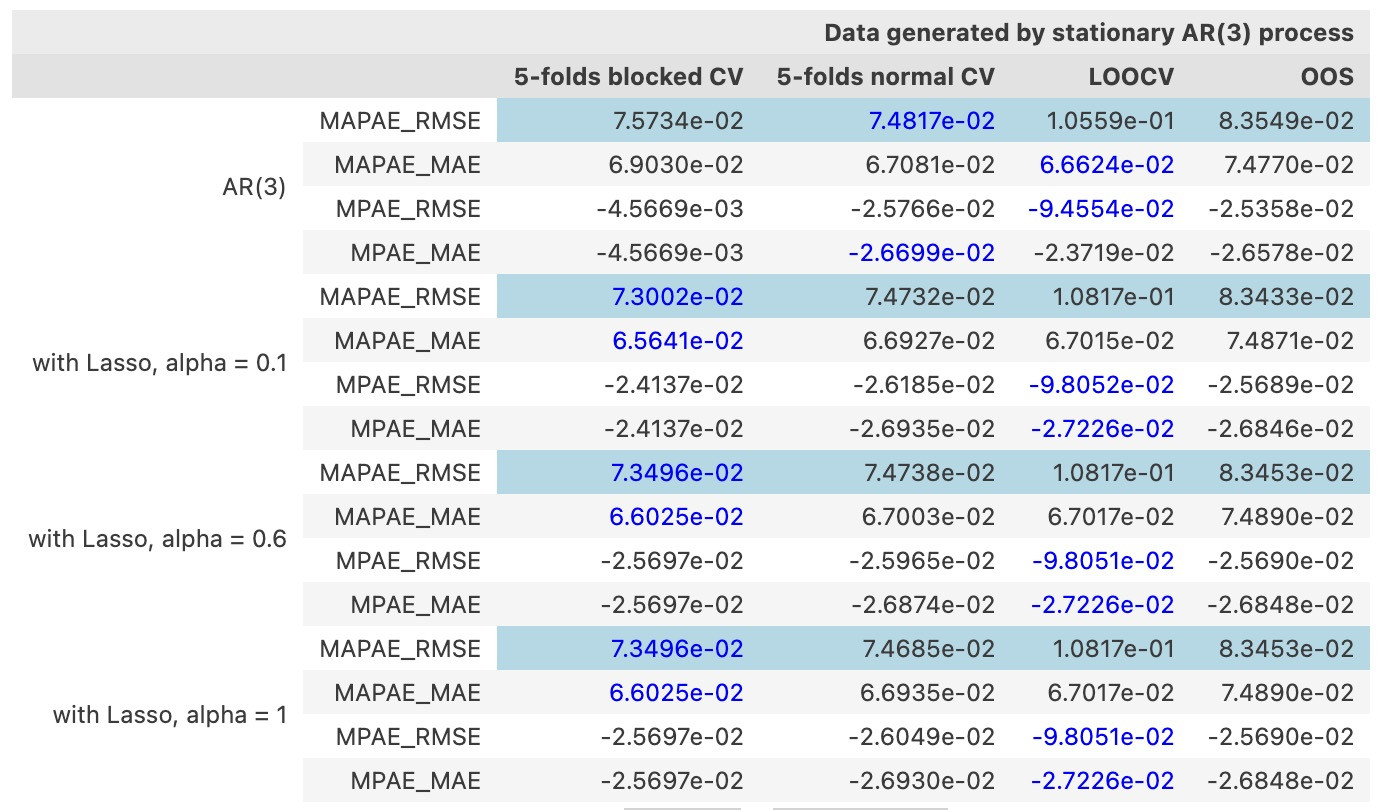
\includegraphics[scale=0.3]{Report/Figures/ar3_table.jpg}
    \label{ar3_table}
\end{figure}
\FloatBarrier

\begin{figure}[hbt!]
    \caption{Experiment 2}
    \centering
    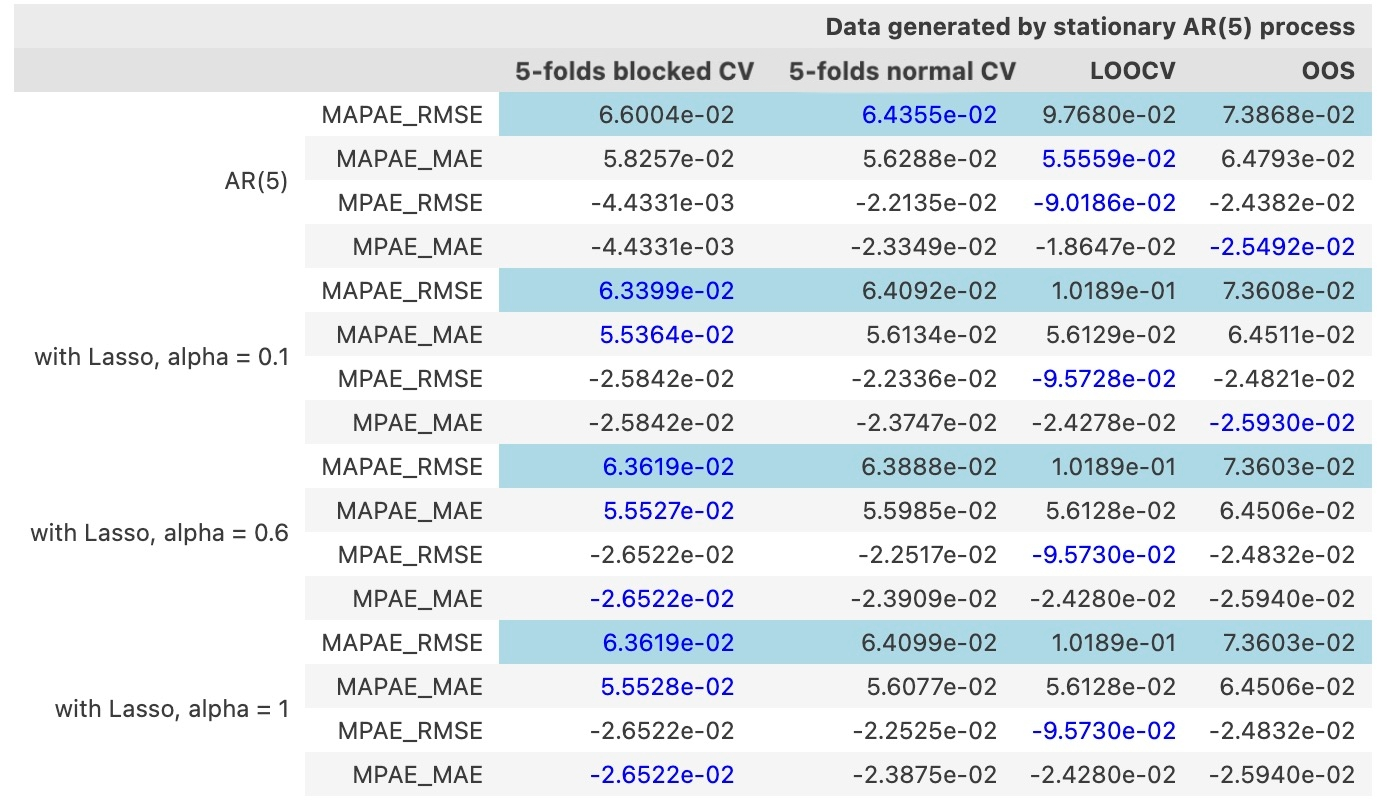
\includegraphics[scale=0.6]{Report/Figures/ar5_table.jpg}
    \label{ar5_table}
\end{figure}
\FloatBarrier

\begin{figure}[hbt!]
    \caption{Experiment 3}
    \centering
    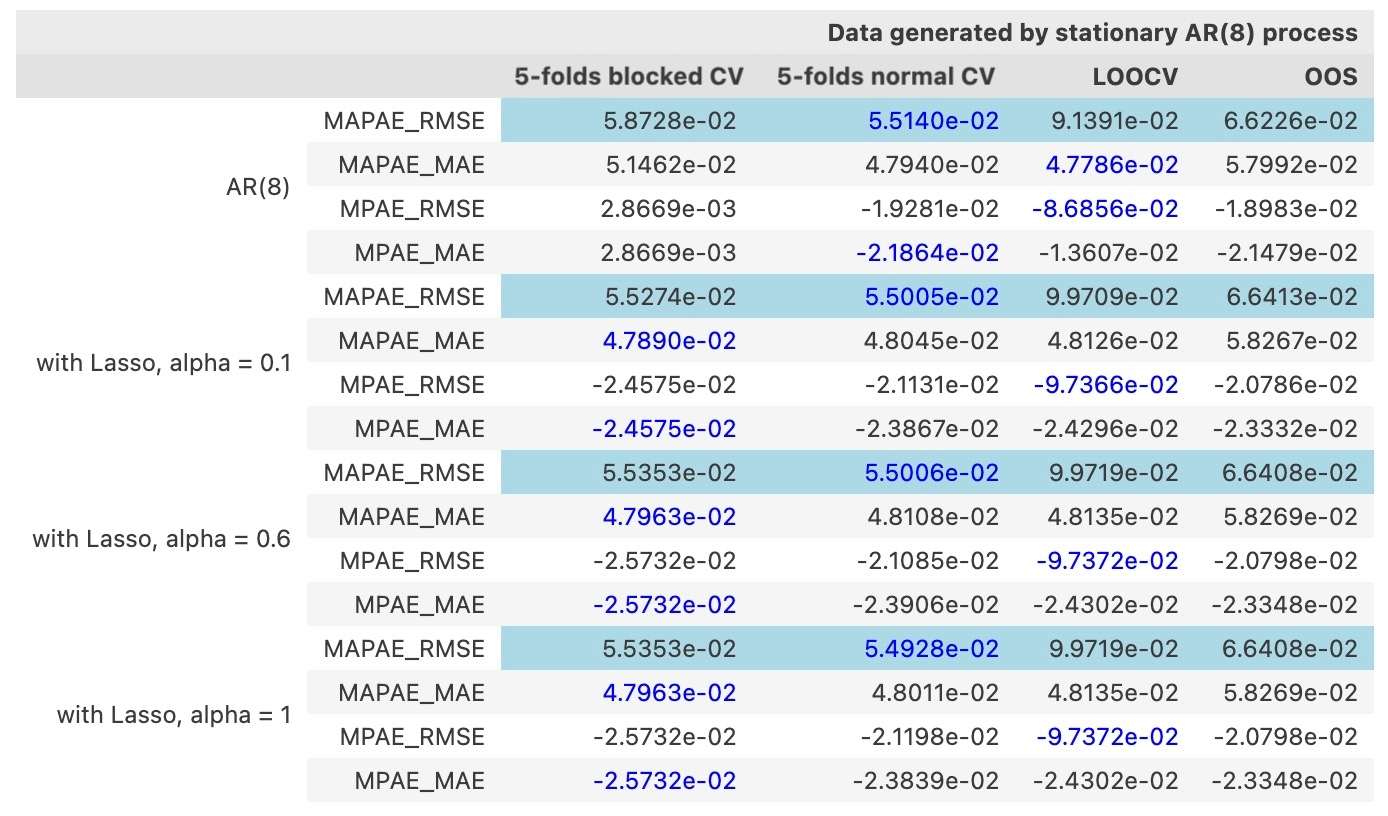
\includegraphics[scale=0.6]{Report/Figures/ar8_table.jpg}
    \label{ar8_table}
\end{figure}
\FloatBarrier


In addition to the error comparison table, we created violin plots to illustrate the distribution of absolute errors of 1000 trials; the absolute error here means the absolute difference between in-set errors and out-set errors. Each "violin" represents the absolute error distribution between $PE$ and $\hat{PE}$ for a specific method (e.g., $LOOCV$), 2 specific models (e.g., AR(3) 
and AR(3) Lasso with $\alpha = 0.6$) and a specific error measure (e.g., \textbf{RMSE}). The width reflects density, with wider sections indicating more frequent errors, and the boxplot inside summarizes the error statistics. The blue diamond marks the mean for the AR model, while the red diamond represents the AR Lasso model. The results, shown in Figures \ref{ar3_v1} to \ref{ar8_v2}, indicate that Blocked CV and Normal CV have a higher frequency of errors near zero compared to $LOOCV$ and $OOS$, especially for \textbf{RMSE} over \textbf{MAE}. Additionally, the Lasso term appears most effective in Blocked CV, as seen by the asymmetry in its violin plot.

\begin{figure}[hbt!]
    \caption{Experiment 1: RMSE between $PE$ and $\hat{PE}$}
    \centering
    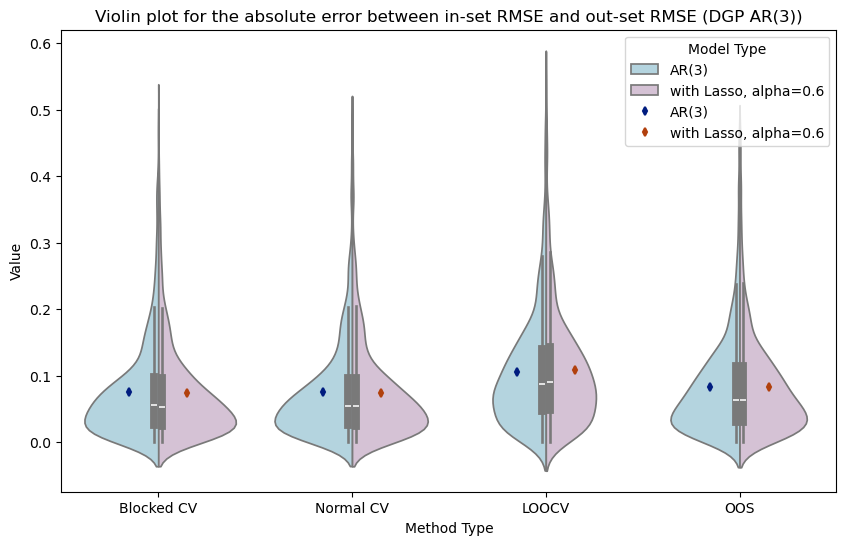
\includegraphics[scale=0.5]{Report/Figures/ar3_violin_rmse.jpg}
    \label{ar3_v1}
\end{figure}
\FloatBarrier

\begin{figure}[hbt!]
    \caption{Experiment 1: MAE between $PE$ and $\hat{PE}$}
    \centering
    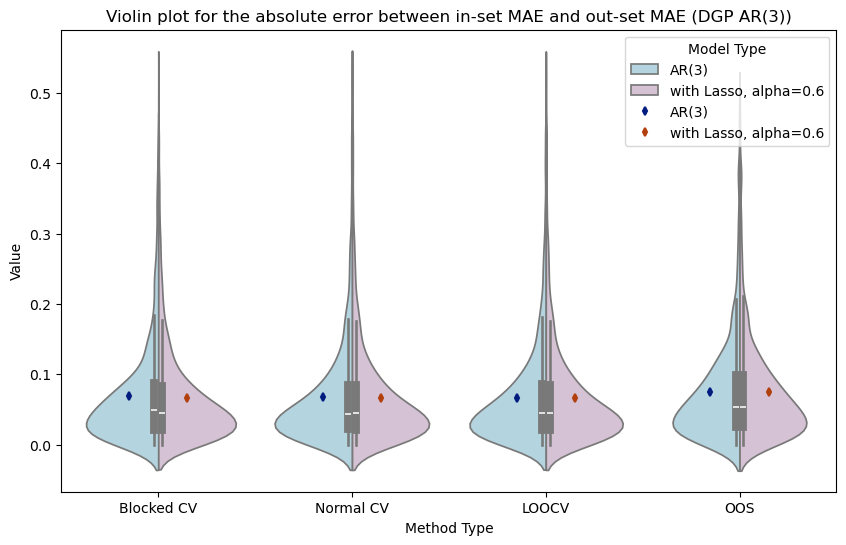
\includegraphics[scale=0.5]{Report/Figures/ar3_violin_mae.jpg}
    \label{ar3_v2}
\end{figure}
\FloatBarrier

\begin{figure}[hbt!]
    \caption{Experiment 2: RMSE}
    \centering
    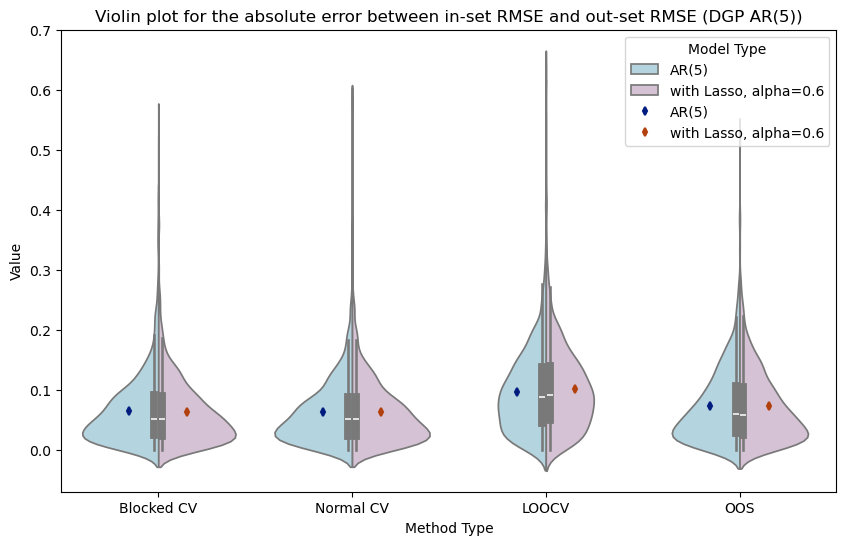
\includegraphics[scale=0.5]{Report/Figures/ar5_violin_rmse.jpg}
    \label{ar5_v1}
\end{figure}
\FloatBarrier

\begin{figure}[hbt!]
    \caption{Experiment 2: MAE}
    \centering
    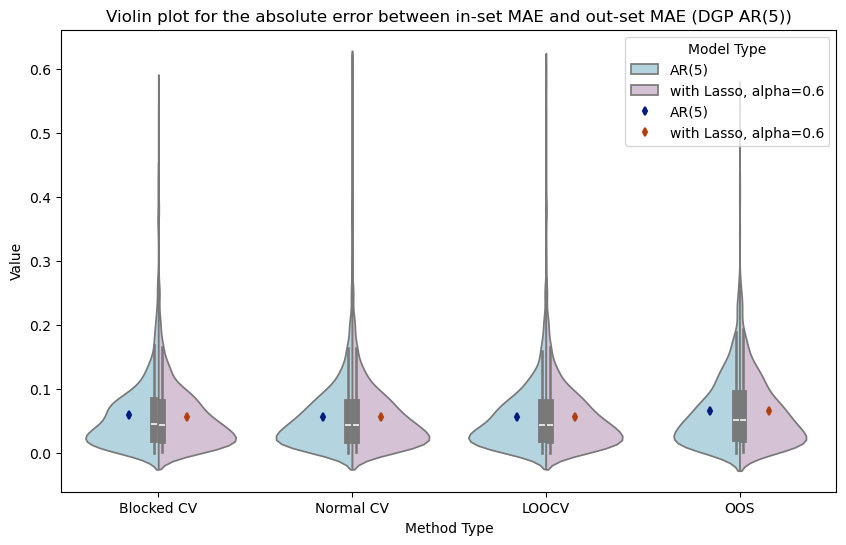
\includegraphics[scale=0.5]{Report/Figures/ar5_violin_mae.jpg}
    \label{ar5_v2}
\end{figure}
\FloatBarrier

\begin{figure}[hbt!]
    \caption{Experiment 3: RMSE}
    \centering
    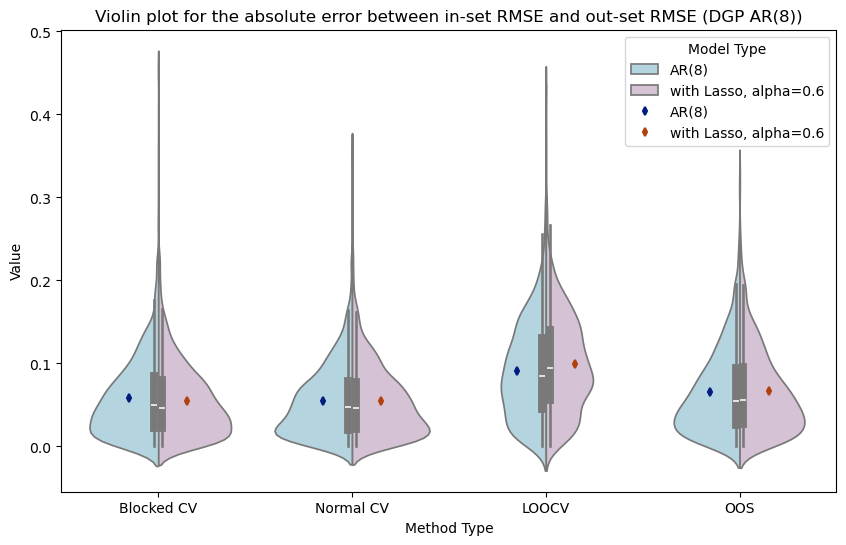
\includegraphics[scale=0.5]{Report/Figures/ar8_violin_rmse.jpg}
    \label{ar8_v1}
\end{figure}
\FloatBarrier

\begin{figure}[hbt!]
    \caption{Experiment 3: MAE}
    \centering
    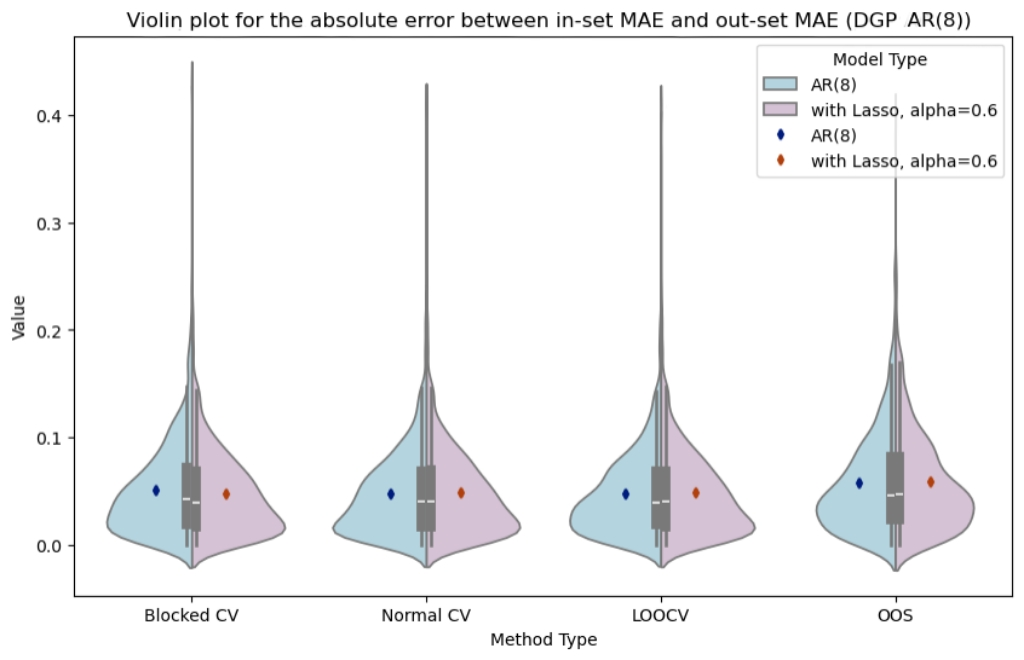
\includegraphics[scale=0.41]{Report/Figures/ar8_violin_mae.jpg}
    \label{ar8_v2}
\end{figure}
\FloatBarrier


\subsection{Future Improvements}
We can extend our study for future improvements in several different aspects and directions. In this section, we discuss five potential improvements to our current experimental design and methodology. These improvements aim for better generalization and error estimation for applications on time series models. 
\\
\\
\underline{Choice of Lasso Parameters}:
Besides testing with a limited and fixed set of $\alpha$ values as we did in our experiments, we can also use cross-validation within the in-set data to automatically select the optimal $\alpha$ value. And we can simulate the process for each Monte Carlo trial to see if a general range of $\alpha$ values out-performs for the chosen fitting model. 
\\
\\
\underline{Extension to Ridge Regression}: Ridge regression is another regularization technique like Lasso, but instead of penalizing the sum of the absolute values of the coefficients (Lasso), Ridge regression penalizes the sum of the squared values of the coefficients. The key difference is that Ridge regression introduces L2 regularization, which shrinks coefficients but does not necessarily set them to zero (as Lasso might do). We can use similar experiments set-up to compare with the results of Lasso regression.
\\
\\
\underline{Extension to Other Time Series Models}: We can extend our simulation to different time series models for data generation process and fitting procedure. However, when using complex models, we should always check if they meet the required assumptions. 
\\
\\
\underline{Other Error Metrics}:
We can explore using different error measures on in-set cross validation and out-set data. During the experiment, we observed a vast range of values for \textbf{RMSE} and \textbf{MAE} when using different scaling factors for the time series data. Using error measures like the percentage error might provide a more standard performance evaluation, since it normalizes the error value according to the data's value range. We can also explore additional measures like \textbf{BIC} or \textbf{AIC} to see how the model complexity affects the generalization error across different fitting methods. We can investigate on how much regularization or model selection improves the model’s ability to generalize.
\\
\\
\underline{Model Interpretability}:
As Lasso can drive some coefficients to zero, it would be interesting to track on how many coefficients are reduced to zero across trials. This would provide some insights on how effective Lasso is and to identify any irrelevant lags. 
\clearpage
\printbibliography
\end{document}

